\pagebreak
\section*{Attention Visualizations}\label{sec:viz-att}
\begin{figure*}[h]
{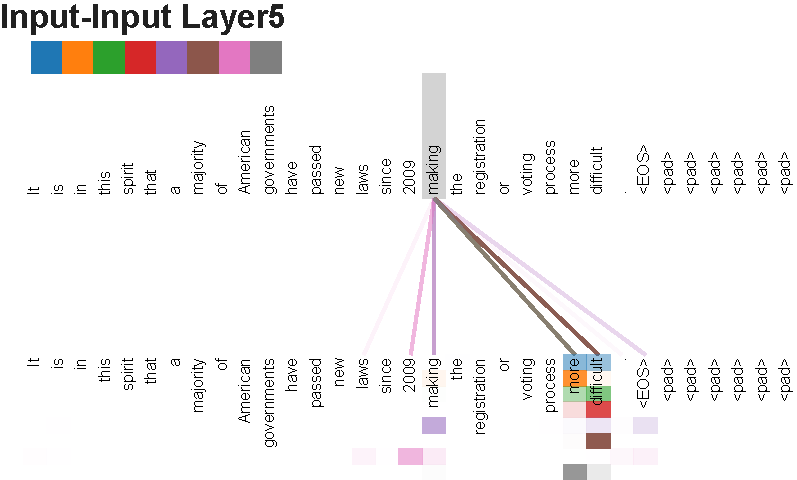
\includegraphics[width=\textwidth, trim=0 0 0 36, clip]{./vis/making_more_difficult5_new.pdf}}
\caption{An example of the attention mechanism following long-distance dependencies in the encoder self-attention in layer 5 of 6. Many of the attention heads attend to a distant dependency of the verb `making', completing the phrase `making...more difficult'.  Attentions here shown only for the word `making'. Different colors represent different heads. Best viewed in color.}
\end{figure*}

\begin{figure*}
{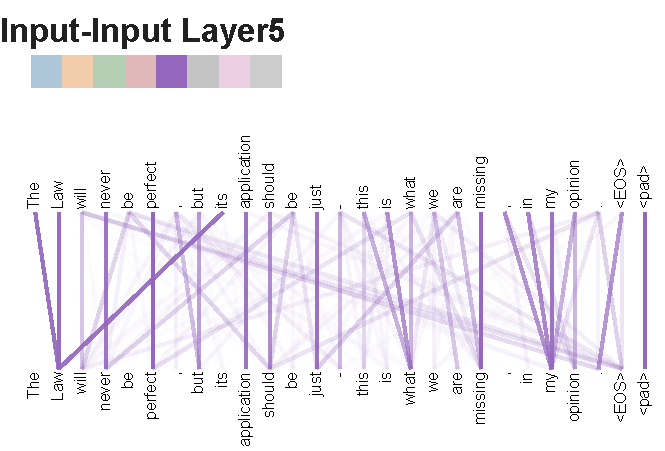
\includegraphics[width=\textwidth, trim=0 0 0 45, clip]{./vis/anaphora_resolution_new.pdf}}
{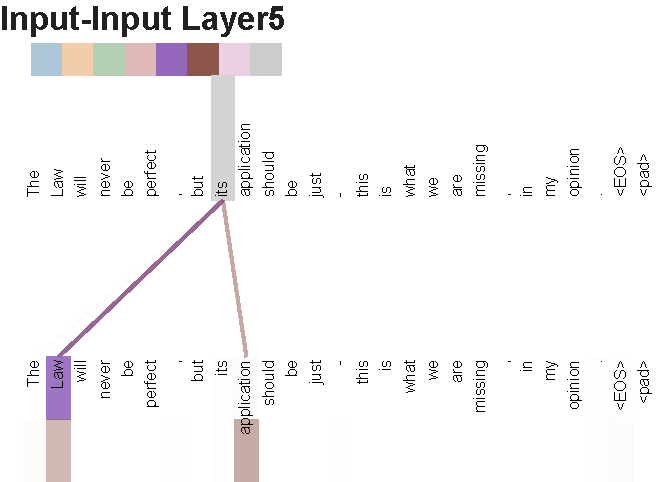
\includegraphics[width=\textwidth, trim=0 0 0 37, clip]{./vis/anaphora_resolution2_new.pdf}}
\caption{Two attention heads, also in layer 5 of 6, apparently involved in anaphora resolution. Top: Full attentions for head 5. Bottom: Isolated attentions from just the word `its' for attention heads 5 and 6. Note that the attentions are very sharp for this word.}
\end{figure*}

\begin{figure*}
{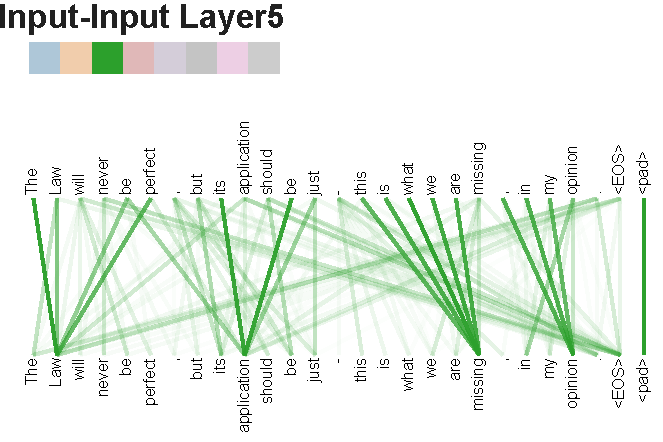
\includegraphics[width=\textwidth, trim=0 0 0 36, clip]{./vis/attending_to_head_new.pdf}}
{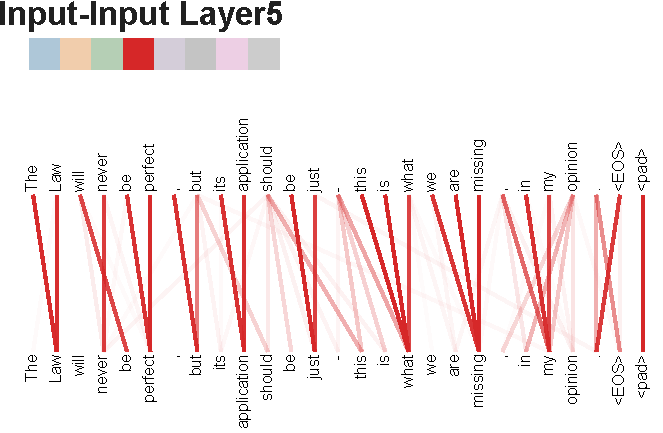
\includegraphics[width=\textwidth, trim=0 0 0 36, clip]{./vis/attending_to_head2_new.pdf}}
\caption{Many of the attention heads exhibit behaviour that seems related to the structure of the sentence. We give two such examples above, from two different heads from the encoder self-attention at layer 5 of 6. The heads clearly learned to perform different tasks.}
\end{figure*}
